\documentclass[aspectratio=169]{beamer}

\usepackage[brazil]{babel}
\usepackage[utf8]{inputenc}
\usepackage[T1]{fontenc}

\usetheme{Madrid}

\setbeamertemplate{navigation symbols}{}

\title[Gestão Organizacional]{Gestão Organizacional}

\author[Diego S. C. Nascimento]{Diego Silveira Costa Nascimento}

\institute[IFRN]{
	Instituto Federal de Educação, Ciência e Tecnologia do Rio Grande do Norte\\
	Campus Natal -- Cidade Alta\\
	diego.nascimento@ifrn.edu.br
}

\date[\today]{\today}

\begin{document}

\begin{frame}[plain]
	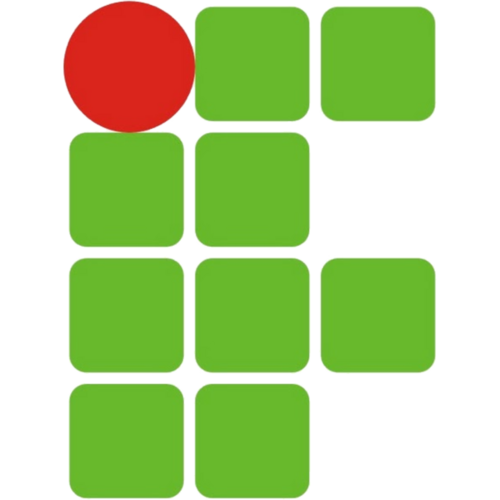
\includegraphics[scale=0.2]{img/IFRN}
	\titlepage
\end{frame}

\logo{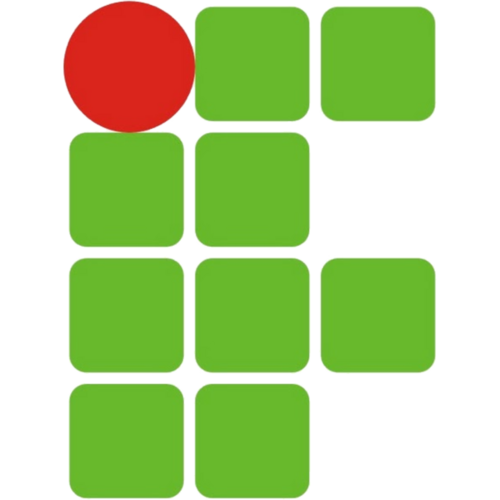
\includegraphics[scale=0.1]{img/IFRN}}

\AtBeginSection[]{
	\begin{frame}
		\frametitle{Sumário}
		\tableofcontents[currentsection]
	\end{frame}
}

\section{Administra\c cão}

\begin{frame}
	\frametitle{Administrar}

	\begin{block}{Origem}
	 Do latim \textit{ad} (dire\c cão) e \textit{minister} (subordina\c cão ou obediência).
	\end{block}
\end{frame}

\begin{frame}
	\frametitle{História}

	\begin{itemize}
		\item 3.000 a.C, Mesopotâmia -- Civiliza\c cão Suméria. Escritura\c cão de opera\c cões comerciais. Primeiros dirigentes e funcionários administrativos profissionais; 
		\item Século XXVI a.C., Egito -- Constru\c cão da grande pirâmide. Planejamento, organiza\c cão e controle elaborados. Primeiro ``livro'' de administra\c cão da história: Deveres do Vizir, gravados em hieróglifos;
		\item VIII a.C. até IV A.D., Império Romano -- Grande organiza\c cão multinacional com institui\c cões administrativas sofisticadas. Diversos tipos de dirigentes, participa\c cão popular no governo, legisla\c cão, estrutura, exército organizado e profissionalizado. Romanos foram precursores das organiza\c cões modernas;
		\item V a.C., Grécia -- Democracia, ética, qualidade, método científico, teoriza\c cão, estratégia, conhecimento e outras ideias fundamentais;
	\end{itemize}
\end{frame}

\begin{frame}
	\frametitle{História}

	\begin{itemize}
		\item 300 a.C, Índia -- Arthashastra de Kautilya, manual de deveres do rei e de seus ministros. Primeiro manual completo de administra\c cão da história;
		\item IV a.C., China -- Sun Tzu, A Arte da Guerra. Manual de estratégia e princípios de comportamento gerencial;
		\item XV - XVI A.D., Itália -- Renascimento. Arsenal de Veneza. Inven\c cão da contabilidade. O Príncipe de Maquiavel. Homem polimático. Capitalismo mercantil. Economia criativa.
		\item XVIII, Inglaterra -- Revolu\c cão industrial;
		\item XIX - XX, Alemanha -- Psicologia experimental. Burocracia;
		\item 1881, Estados Unidos -- Primeira escola de administra\c cão;
		\item Transi\c cão para o Século XX, Estados Unidos -- Início do movimento da administra\c cão científica. Linha do montagem móvel. Movimento da qualidade;
	\end{itemize}
\end{frame}

\begin{frame}
	\frametitle{História}

	\begin{itemize}
		\item 1916, Fran\c ca -- Administra\c cão Industrial e Geral;
		\item Sistema Toyota de Produ\c cão. Administra\c cão enxuta. Modelo Japonês de administra\c cão.
		\item 1969, Estados Unidos -- Funda\c cão do PMI; e
		\item Década de 1980, Estados Unidos -- Reengenharia. Seis Sigmas. Redesenho de processo.
	\end{itemize}
\end{frame}

\begin{frame}
	\frametitle{O que é Teoria Geral da Administra\c cão?}

	\begin{block}{Defini\c cão}
	É o conjunto de conhecimentos a respeito das organiza\c cões e do processo de administrá-las, sendo composta por princípios, proposi\c cões e técnicas em permanente elabora\c cões.
	\end{block}
\end{frame}

\begin{frame}
	\frametitle{Frederick Taylor}

	\begin{itemize}
		\item Liderou o movimento da administra\c cão científica;
		\item Nascido nos Estados Unidos;
		\item Para determinar a melhor forma de executar um trabalho, dividiu cada atividades em movimentos menores e cronometrou cada um deles;
		\item Analisou a a\c cão para eliminar movimentos desnecessários, o que dava a origem ao método mais ágil e eficiente de executar uma tarefa atribuída;
		\item Traz os conceitos de eficácia e eficiência no meio da produ\c cão industrial.
	\end{itemize}
\end{frame}

\begin{frame}
	\frametitle{Eficácia vs Eficiência}

\begin{columns}
	\column{0.5\textwidth}

	\structure{Eficácia}
	\begin{itemize}
		\item Fazer as coisas certas;
		\item Preocupa\c cão com os fins;
		\item Ênfase nos resultados; e
		\item Maximizar os objetivos.
	\end{itemize}
		
	\column{0.5\textwidth}

	\structure{Eficiência}
	\begin{itemize}
		\item Fazer bem as coisas;
		\item Preocupa\c cão com os meios;
		\item Ênfase no processo; e
		\item Ausência de desperdícios.
	\end{itemize}
\end{columns}

\end{frame}

\begin{frame}
	\frametitle{Teoria Científica de Taylor}

	\begin{itemize}
		\item Mecanicismo;
		\item Superespecializa\c cão do trabalhador;
		\item Visão microscópica do homem;
		\item Abordagem de sistema fechado; e
		\item A explora\c cão dos empregados.
	\end{itemize}
\end{frame}

\begin{frame}
	\frametitle{Henry Ford}

	\begin{itemize}
		\item Foi um empresário norte-americano;
		\item Fundador da Ford Motor Company; e
		\item Desenvolveu e implantou a linha de montagem em série.
	\end{itemize}
\end{frame}

\begin{frame}
	\frametitle{Princípios de Ford }

	\begin{itemize}
		\item Princípio da intensifica\c cão;
		\item Princípio da economicidade; e
		\item Princípio da produtividade.
	\end{itemize}
\end{frame}

\begin{frame}
	\frametitle{Henri Fayol}

	\begin{itemize}
		\item Nascido na Fran\c ca;
		\item Foi fundador da teoria clássica da administra\c cão;
		\item Foi o primeiro a tratar a administra\c cão como disciplina para formar lidenra\c cas qualificadas;
		\item Toma como base a busca por máxima eficiência através da visão homem econômico;
		\item Ou seja, considera o homem como racional e com focos racionais;
		\item Criou um sistema para otimizar a gerência dando a cada gerente o seus deveres.
	\end{itemize}
\end{frame}

\begin{frame}
	\frametitle{Fun\c cões Administrativas de Fayol}

	\begin{itemize}
		\item Planejar;
		\item Organiza\c cão;
		\item Dire\c cão; e
		\item Controle.
	\end{itemize}
\end{frame}

\begin{frame}
	\frametitle{Max Weber}

	\begin{itemize}
		\item Nascido na Alemanha;
		\item Fundou o método de análise sociológica; e
		\item Lan\c cou as bases para o estudo das organiza\c cões e da burocracia.
	\end{itemize}
\end{frame}

\begin{frame}
	\frametitle{Princípios de Max Weber}

	\begin{itemize}
		\item Indivíduo;
		\item Ética; e
		\item Rela\c cão social.
	\end{itemize}
\end{frame}

\section{Estratégia}

\begin{frame}
	\frametitle{Estratégia}

	\begin{block}{Defini\c cão}
		``Strategy explains how an organization, faced with competition, will achieve superior performance'' (Michael Porter)
	\end{block}
\end{frame}

\begin{frame}
	\frametitle{Ferramenta de Estratégia de Negócio}

	\begin{enumerate}
		\item Missão;
		\item Visão; e
		\item Valores.
	\end{enumerate}
\end{frame}

\begin{frame}
	\frametitle{Missão}

	\begin{block}{Defini\c cão}
		É o propósito da empresa existir.
	\end{block}\vfill
	
	\begin{exampleblock}{Exemplo}
		``Satisfazer com excelência a nossos consumidores de bebidas. Ser líder total de bebidas, gerando valor econômico, social e ambiental sustentável, gerenciando modelos de negócio inovadores e ganhadores, com os melhores colaboradores do mundo.'' (Coca-Cola)
	\end{exampleblock}
\end{frame}

\begin{frame}
	\frametitle{Visão}

	\begin{block}{Defini\c cão}
		É a situação em que a empresa deseja chegar (em período definido de tempo).
	\end{block}\vfill

	\begin{exampleblock}{Exemplo}
		``Produzir produtos de alta qualidade e de fácil uso que incorporam alta tecnologia para o indivíduo, provando que alta tecnologia não precisa ser intimidadora para aqueles que não são experts em computação.'' (Apple)
	\end{exampleblock}
\end{frame}

\begin{frame}
	\frametitle{Valores}

	\begin{block}{Defini\c cão}
		São os ideais de atitude, comportamento e resultados que devem estar presentes nos colaboradores e nas relações da empresa com seus clientes, fornecedores e parceiros.
	\end{block}\vfill
	
	\begin{exampleblock}{Exemplo}
		``Humanismo; Criatividade; Equilíbrio; e Transparência.'' (Natura)
	\end{exampleblock}
\end{frame}

\begin{frame}
	\frametitle{Análise de SWOT}

	\begin{block}{Defini\c cão}
		É uma técnica de planejamento estratégico utilizada para auxiliar pessoas ou organizações a identificar forças, fraquezas, oportunidades, e ameaças relacionadas à competição em negócios ou planejamento de projetos.
	\end{block}\vfill
	
	\begin{center}
		\begin{tabular}{| c | c | c |}
			\hline
				Fatores & Positivos & Negativos \\
			\hline 
				Internos & \structure{Strenghts} (For\c cas) &  \structure{Weaknesses} (Fraquezas) \\ 
			\hline
				Externos &\structure{Opportunities} (Oportunicades) & \structure{Threats} (Amea\c cas)\\ 
			\hline
		\end{tabular}
	\end{center}
\end{frame}

\section{Organiza\c cão}

\begin{frame}
	\frametitle{Organiza\c cão}

	\begin{block}{Defini\c cão}
		É um conjunto de pessoas e recursos na busca de uma ou mais objetivos comuns.
	\end{block}
\end{frame}

\begin{frame}
	\frametitle{As quatro fun\c cões da organiza\c cão}

	\begin{itemize}
		\item Produ\c cão;
		\item Marketing;
		\item Recursos humanos; e
		\item Financeiro.
	\end{itemize}
\end{frame}

\begin{frame}
	\frametitle{Níveis Hieráquicos}

	\begin{itemize}
		\item Estratégico (CEOs, presidentes, diretores);
		\item Tático (diretores, gerentes); e
		\item Operacional (supervisores, operadores).
	\end{itemize}
\end{frame}

\begin{frame}
	\frametitle{Metas e Indicadores SMART}

	\begin{block}{Defini\c cão}
		É uma ferramenta utilizada para ajudar as pessoas e empresas a definir e alcançar seus objetivos de maneira clara e eficiente.
	\end{block}
\end{frame}

\begin{frame}
	\frametitle{SMART}

	\begin{itemize}
		\item \underline{S}pecific;
		\item \underline{M}easurable;
		\item \underline{A}ttainable;
		\item \underline{R}elevant; e
		\item \underline{T}ime based.
	\end{itemize}
\end{frame}

\begin{frame}
	\frametitle{Specific}

	\begin{itemize}
		\item O objetivo demarcado deve ser específico;
		\item Deve ser claro; e
		\item Não podem permitir qualquer tipo de interpretação dúbia ou controversa.
	\end{itemize}
\end{frame}

\begin{frame}
	\frametitle{Measurable}

	\begin{itemize}
		\item Todo objetivo poder ser traduzido em números; e
		\item No momento da definição do seu objetivo, analise se o mesmo poderá ser, sistematicamente, interpretado e manipulado numericamente.
	\end{itemize}
\end{frame}

\begin{frame}
	\frametitle{Attainable}

	\begin{itemize}
		\item As metas devem seguir uma razoabilidade;
		\item Todos devem concordar com o estabelecimento deste indicador; e
		\item O ambiente externo a organiza\c cão deve ser favorável.
	\end{itemize}
\end{frame}

\begin{frame}
	\frametitle{Relevant}

	\begin{itemize}
		\item O indicardor deve estar alinhado com o objetivo da organiza\c cão;
		\item Deve existir consonância do objetivo com os ideais e valores defendidos; e
		\item Deve existir real disposição da equipe para se engajar no projeto.
	\end{itemize}
\end{frame}

\begin{frame}
	\frametitle{Time based}

	\begin{itemize}
		\item Consiste na referenciação temporal do objetivo;
		\item Definição um prazo para a realização e cumprimento do objetivo;
		\item Cria um senso de urgência indispensável para o sucesso de um projeto; e
		\item Evita procrastinação e desorganização operacional.
	\end{itemize}
\end{frame}

\begin{frame}
	\frametitle{Canva}

	\begin{block}{Defini\c cão}
		É uma ferramenta dinâmica em formato de um quadro que permite analisar o modelo de negócios que está sendo criado, remodelado ou adaptado.
	\end{block}
\end{frame}

\begin{frame}
	\frametitle{Quadro}
	
	\begin{center}
			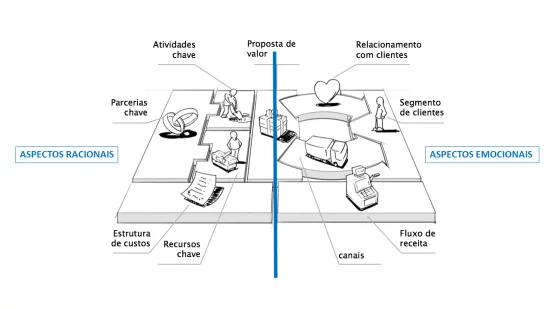
\includegraphics[scale=0.7]{img/canva}
	\end{center}
\end{frame}

\begin{frame}
	\frametitle{Blocos}

	\begin{enumerate}
		\item Segmento de clientes;
		\item Proposta de valor;
		\item Canais;
		\item Relacionamento com clientes;
		\item Fontes de receita;
		\item Recursos principais;
		\item Atividades-chave;
		\item Parcerias principais; e
		\item Estrutura de custos.
	\end{enumerate}
\end{frame}

\begin{frame}
	\frametitle{Segmento de clientes}

	\begin{block}{Defini\c cão}
		 Define os diferentes grupos de pessoas ou organizações que uma empresa busca alcançar e atender.
	\end{block}
\end{frame}

\begin{frame}
	\frametitle{Proposta de valor}

	\begin{block}{Defini\c cão}
		 Descreve o conjunto de razões pelas quais seu cliente irá optar pelo seu produto ou serviço.
	\end{block}
\end{frame}

\begin{frame}
	\frametitle{Canais}

	\begin{block}{Defini\c cão}
		 Descreve por onde seu negócio se comunica, distribui e vende o produto ou serviço aos seus clientes.
	\end{block}
\end{frame}

\begin{frame}
	\frametitle{Relacionamento com clientes}

	\begin{block}{Defini\c cão}
		 Descreve as formas e os meios que você vai estabelecer para criar ou manter a relação com seus clientes.
	\end{block}
\end{frame}

\begin{frame}
	\frametitle{Fontes de receita}

	\begin{block}{Defini\c cão}
		 Representa o dinheiro que sua empresa vai gerar através da venda do seu produto e serviço, e também as formas com que você irá capturar esse valor.
	\end{block}
\end{frame}

\begin{frame}
	\frametitle{Recursos principais}

	\begin{block}{Defini\c cão}
		 Descreve os recursos mais importantes para fazer seu modelo de negócios funcionar.
	\end{block}
\end{frame}

\begin{frame}
	\frametitle{Atividades-chave}

	\begin{block}{Defini\c cão}
		 Descreve as ações mais importantes que seu negócio deve realizar para fazer o modelo de negócios funcionar.
	\end{block}
\end{frame}

\begin{frame}
	\frametitle{Parcerias principais}

	\begin{block}{Defini\c cão}
		 Refere-se à rede de fornecedores e parceiros, ou seja, empresas, pessoas e entidades que são seus aliados na otimização e redução de risco do negócio.
	\end{block}
\end{frame}

\begin{frame}
	\frametitle{Estrutura de custos}

	\begin{block}{Defini\c cão}
		 Diz respeito a todos os custos envolvidos na operação do seu modelo de negócios.
	\end{block}
\end{frame}

\end{document}